\section{Tổng quan sản phẩm}
\subsection{Bối cảnh sản phẩm}
\quad Phần này cung cấp cái nhìn tổng quan về các khả năng của sản phẩm, giao tiếp với các ứng dụng khác và cấu hình hệ thống. AutoEye là đặc tả và hiện thực hóa một hệ thống đề xuất nhằm theo dõi phương tiện và phân loại trạng thái giao thông ngay trên thiết bị, áp dụng cho một đoạn đường cụ thể. Hệ thống hướng tới việc thiết kế một giải pháp chi phí thấp, hiệu suất cao, triển khai các thuật toán học máy ngay trên thiết bị, nhằm hỗ trợ khả năng mở rộng theo chiều ngang khi áp dụng vào hạ tầng ở cấp độ thành phố.

\subsection{Các giả định và sự phụ thuộc}
\quad Những sự giả định và phụ thuộc của AutoEye bao gồm:


\begin{itemize}
    \item \textbf{Môi trường vận hành:} Giả định rằng AutoEye sẽ được triển khai trên các vi xử lý có tài nguyên hạn chế nghiêm trọng, với dung lượng bộ nhớ dưới 512 KiB và bộ nhớ flash chỉ cho phép đọc. Hệ thống cũng bao gồm một phía máy chủ, có chức năng giám sát và tổng hợp các kết quả được báo cáo từ các vi xử lý đã triển khai, nhằm cung cấp góc nhìn phân tích dữ liệu.
    
    \item \textbf{Phụ thuộc bên ngoài:} AutoEye được thiết kế nhằm xây dựng một hệ thống lưu trữ và truyền thông dữ liệu hoàn chỉnh, không phụ thuộc vào các thành phần hoặc dịch vụ bên ngoài.
    
    \item \textbf{Khả năng mở rộng:} Hệ thống được giả định có thể xử lý hiệu quả một lượng nhỏ dữ liệu trong khoảng thời gian định sẵn. Mỗi thiết bị biên (edge unit) phải tự thực hiện các tác vụ theo dõi và phân loại mà không cần chuyển giao việc xử lý cho các thiết bị khác.
\end{itemize}

\quad \textbf{Nếu những yếu tố này thay đổi, có thể sẽ cần điều chỉnh hoặc cập nhật Tài liệu Tổng quan để đáp ứng các yêu cầu mới.}

\subsection{Kiến trúc hệ thống}

\subsubsection{Sơ đồ kiến trúc hệ thống}



\begin{figure}[H]
    \centering
    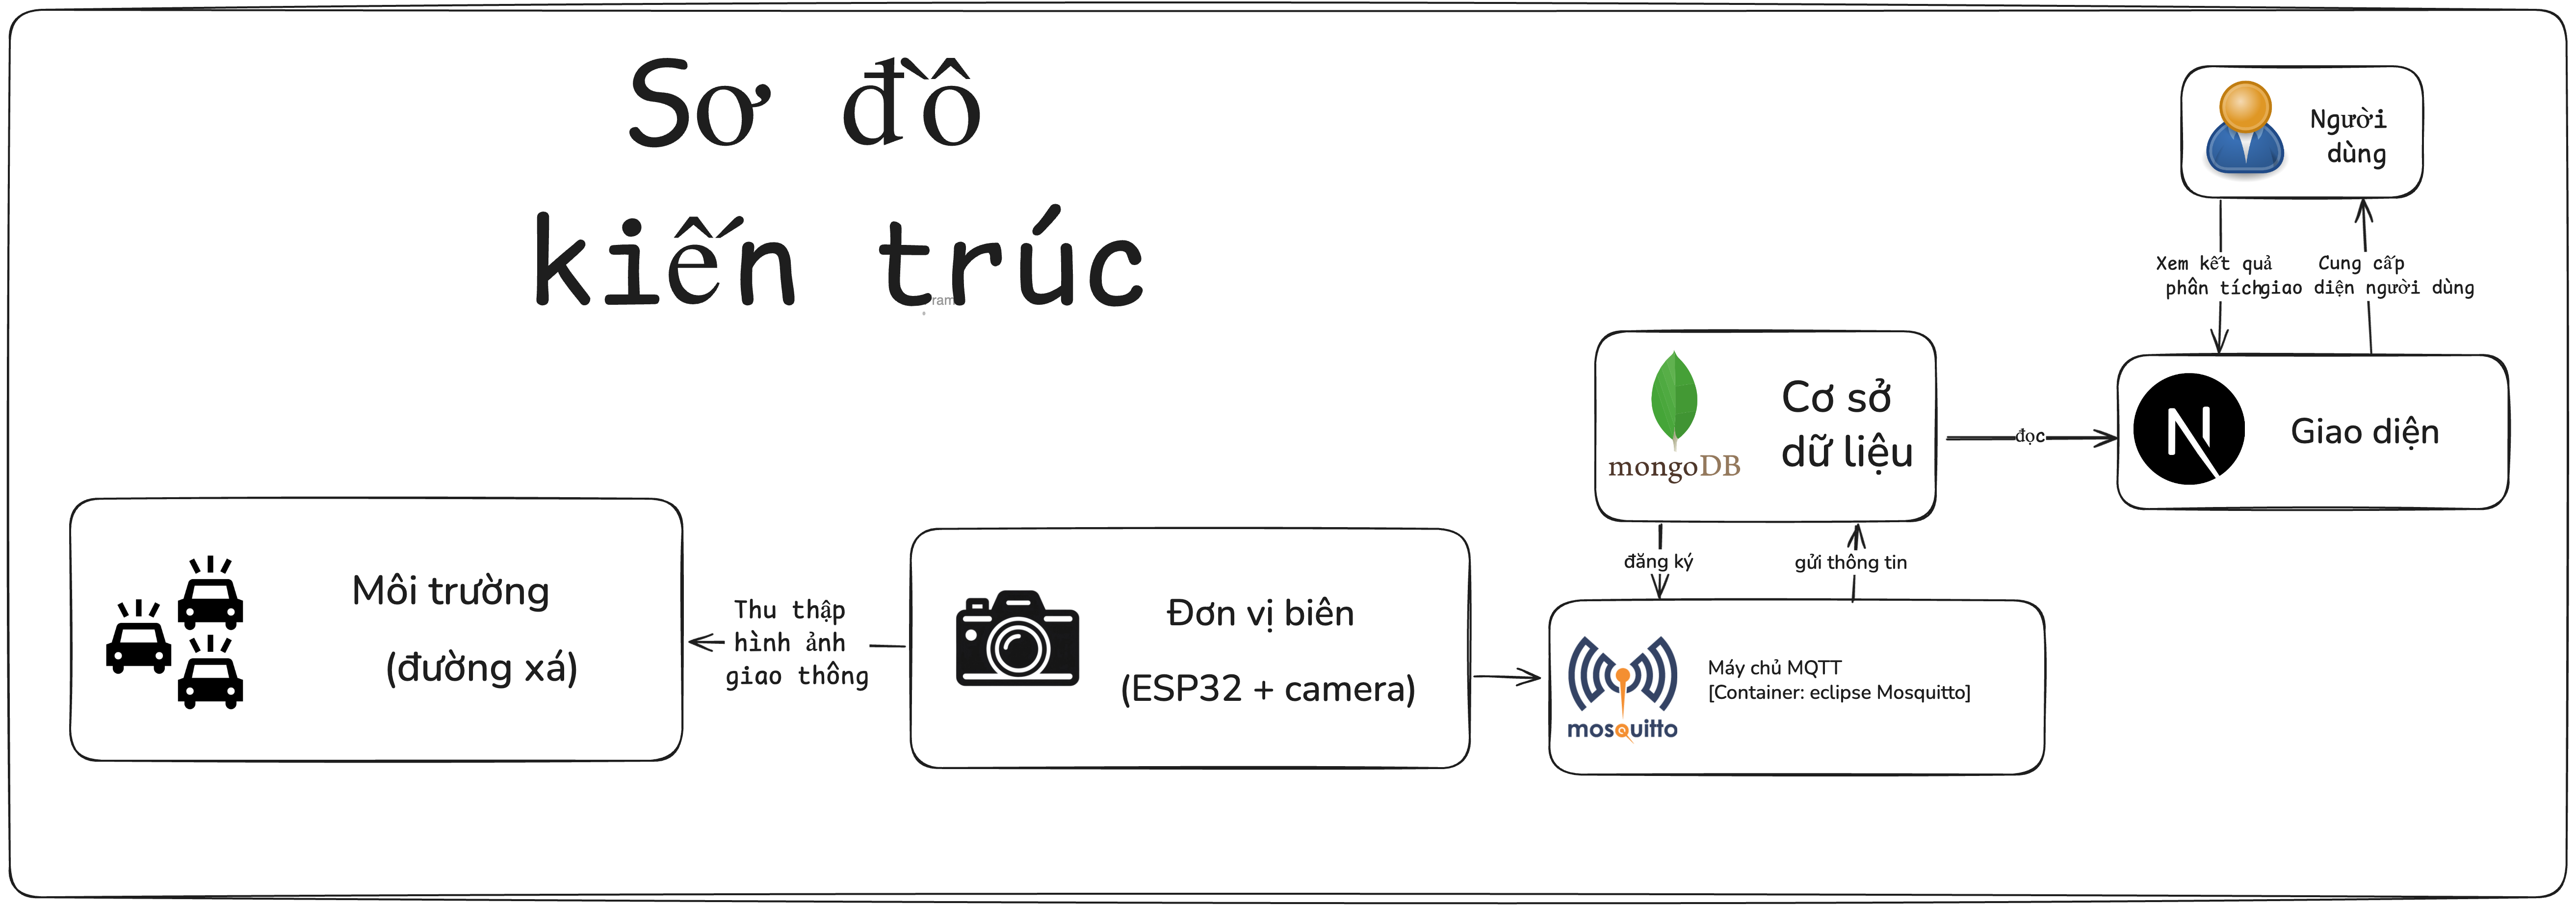
\includegraphics[width=1\textwidth]{image/architecture.png}
    \caption{Sơ đồ hệ thống}
    \label{fig:architecture}
\end{figure}



\quad Kiến trúc hệ thống chung của AutoEye bao gồm các đơn vị edge trực tiếp thu thập dữ liệu từ môi trường và phân tích dữ liệu để đưa ra các thông tin về lưu lượng xe, tình trạng ùn tắc giao thông tại các con đường.

\quad Các đơn vị edge sẽ độc lập xử lý dữ liệu của khu vực mà nó được phân bổ để giải quyết. Các kết quả từ mỗi đơn vị edge sẽ được gửi đến một máy chủ trung tâm thông qua giao thức MQTT. Thông tin gửi đến của mỗi đơn vị edge sẽ bao gồm chỉ số định danh của đơn vị edge, thời gian gửi, lượng xe tại thời điểm đó và tình trạng ùn tắc giao thông. Các dữ liệu này sẽ được lưu trữ tạm thời trên máy chủ MQTT.

\quad Sau mỗi khoảng thời gian T, một máy chủ khác sẽ yêu cầu lượng dữ liệu đang được chứa trong hàng chờ của máy chủ MQTT thông qua giao thức HTTP. Máy chủ này mang vai trò quản lý xuất-nhập của dữ liệu vừa thu được từ các đơn vị edge thông qua máy chủ MQTT với một cơ sở dữ liệu; đồng thời cung cấp và tương tác với giao diện người dùng khi cần thiết. Máy chủ cho phép xem tình trạng mới nhất của mỗi đơn vị edge, bao gồm cả các đơn vị có thể mất kết nối. Ngoài ra, máy chủ còn cho phép truy xuất các thông tin đã được lưu lại từ trước.

\subsubsection{Sơ đồ các đơn vị edge}

\begin{figure}[H]
    \centering
    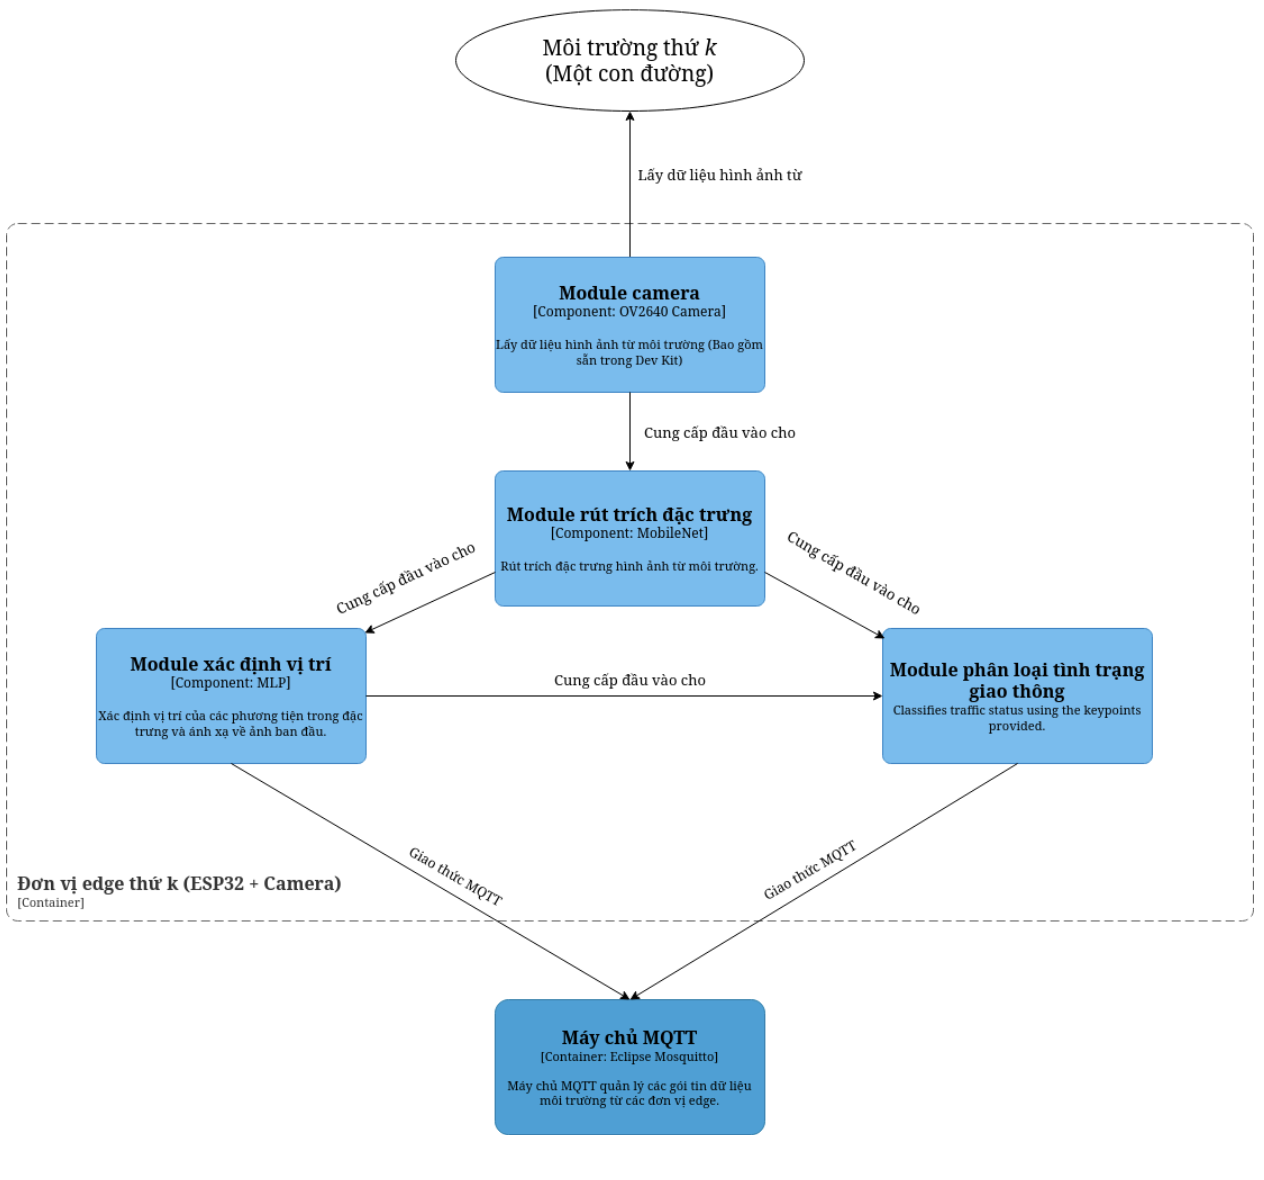
\includegraphics[width=0.85\textwidth]{image/modules.png}

    \label{fig:edges}
\end{figure}

\quad Các đơn vị edge có vai trò thu thập các dữ liệu của môi trường đang hoạt động (là các con đường) thông qua module camera OV2640. 

\quad Sau đó, các đơn vị edge sẽ độc lập sử dụng mô hình MobileNet cùng với một số các kỹ thuật tối ưu bộ nhớ sử dụng để rút trích và giảm chiều các đặc trưng của các ảnh từ môi trường.

\quad Tiếp theo, đặc trưng từ module rút trích đặc trưng sẽ được cung cấp cho module xác định vị trí (localizer) nhằm dự đoán vị trí của các phương tiện bằng một mạng MLP thông thường.

\quad Đầu ra của module dự đoán vị trí và rút trích đặc trưng sẽ được cung cấp cho module dự đoán trạng thái giao thông. Module dự đoán trạng thái giao thông sẽ tiến hành phân loại tình trạng giao thông theo lưu lượng xe. Cụ thể, module sẽ xét số phương tiện đang lưu hành trong t khung hình gần nhất và tốc độ di chuyển trung vị của các phương tiện đó nhằm xác định tình trạng có ùn tắc giao thông, có nguy cơ ùn tắc giao thông hoặc không có nguy cơ ùn tắc giao thông.

\subsection{Use case Diagram}

\begin{figure}[H]
    \centering
    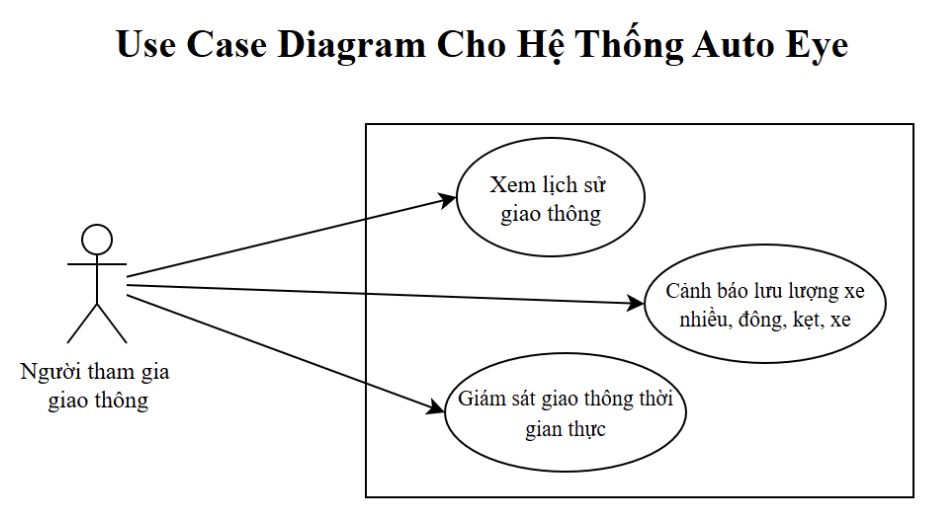
\includegraphics[width=0.85\textwidth]{image/usecase.png}

    \label{fig:usecase}
\end{figure}

\subsubsection{Đặc tả cho từng use case}

\begin{enumerate}
    \item \textbf{Use case 1: Xem lịch sử giao thông}
    
    \begin{table}[H]
        \centering
        \begin{tabular}{|p{4cm}|p{10cm}|}
            \hline
            \textbf{Thành phần} & \textbf{Mô tả} \\ \hline
            Tên & Xem lịch sử giao thông \\ \hline
            Tác nhân & Người tham gia giao thông \\ \hline
            Mục tiêu & Truy xuất dữ liệu lưu lượng phương tiện trong một khoảng thời gian \\ \hline
            Cơ sở dữ liệu & Bảng \texttt{traffic\_log} \\ \hline
        \end{tabular}
    \end{table}
    
    \textbf{Luồng xử lý:}
    \begin{itemize}
        \item Người dùng chọn khu vực cần xem và thời gian cần thống kê (ví dụ: từ 6h đến 9h ngày 28/5).
        \item Hệ thống thực hiện truy vấn đến bảng \texttt{traffic\_log}.
        \item Dữ liệu trả về dưới dạng bảng hoặc biểu đồ đường.
        \item Hiển thị xu hướng lưu lượng xe theo từng khung giờ, từng loại xe.
    \end{itemize}
    
    \item \textbf{Use case 2: Cảnh báo lưu lượng xe nhiều, đông, kẹt xe}
    
    \begin{table}[H]
        \centering
        \begin{tabular}{|p{4cm}|p{10cm}|}
            \hline
            \textbf{Thành phần} & \textbf{Mô tả} \\ \hline
            Tên & Cảnh báo lưu lượng xe nhiều, đông, kẹt xe \\ \hline
            Tác nhân & Người tham gia giao thông \\ \hline
            Mục tiêu & Nhận cảnh báo khi lưu lượng phương tiện vượt quá ngưỡng cho phép \\ \hline
            Cơ sở dữ liệu & Bảng \texttt{traffic\_alerts}, \texttt{thresholds} (mức ngưỡng) \\ \hline
        \end{tabular}
    \end{table}
    \quad Luồng xử lý:
    \begin{itemize}
        \item Sau khi AI model đếm phương tiện, kết quả được so sánh với mức ngưỡng (threshold) theo từng khung giờ/khu vực.
        \item Nếu số lượng xe trong khung giờ vượt quá ngưỡng, hệ thống tạo một bản ghi cảnh báo.
        \item Gửi thông báo (qua API/Telegram/email) đến người dùng hoặc hệ thống dashboard.
        \item Người tham gia giao thông thấy cảnh báo đỏ, khu vực kẹt xe → chủ động thay đổi tuyến đường.
    \end{itemize}
    \item \textbf{Use case 3: Giám sát giao thông thời gian thực}
    \begin{table}[H]
        \centering
        \caption{Use case: Giám sát giao thông thời gian thực}
        \begin{tabular}{|p{4cm}|p{10cm}|}
            \hline
            \textbf{Thành phần} & \textbf{Mô tả} \\ \hline
            Tên & Giám sát giao thông thời gian thực \\ \hline
            Tác nhân & Người tham gia giao thông \\ \hline
            Mục tiêu & Hiển thị số lượng xe đang lưu thông tại một khu vực theo thời gian thực \\ \hline
            Cơ sở dữ liệu & Bảng \texttt{traffic\_log} (ghi lại số lượng xe, thời gian, vị trí) \\ \hline
        \end{tabular}
    \end{table}

    \quad Luồng xử lý:
    \begin{itemize}
        \item Thiết bị ESP32-CAM chụp hình giao thông định kỳ (mỗi 5 giây).
        \item Ảnh được xử lý tại Edge:
        \begin{itemize}
            \item Ảnh được tiền xử lý bóc tách đặc trưng
            \item Model AI nhận diện phương tiện và đếm số lượng
        \end{itemize}
        \item Kết quả được ghi vào DB (traffic\_log với các trường time\_stamp, location\_id, vehicle\_count, vehice\_type).
        \item Người dùng truy cập dashboard để truy xuất dữ liệu traffic\_log gần nhất.
        \item Hiển thị biểu đồ lưu lượng giao thông trực tiếp trên dashboard.

    \end{itemize}


\end{enumerate}
\subsection{Quy trình tự động hoá tích hợp, cập nhật mô hình vào thiết bị}

\begin{figure}[H]
    \centering
    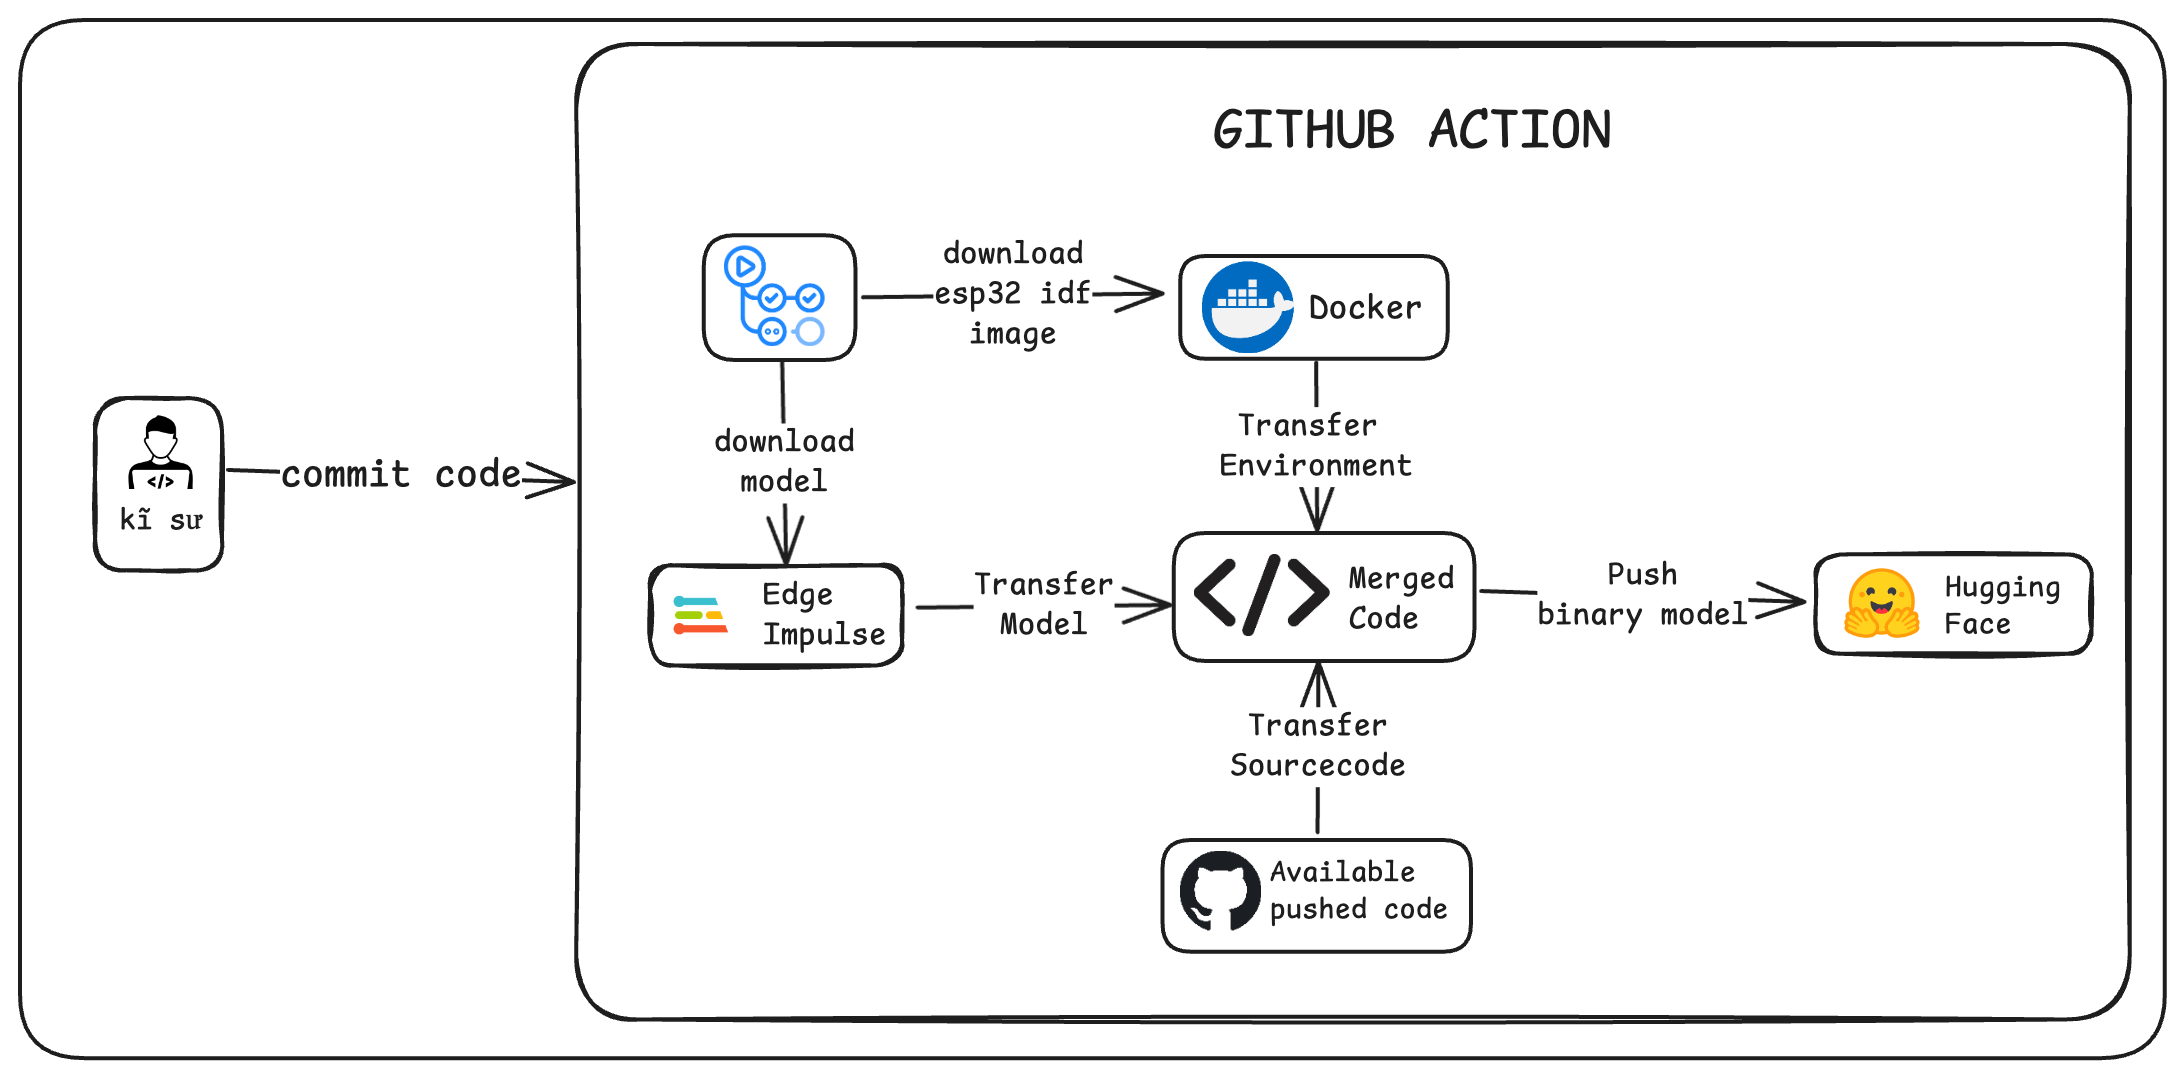
\includegraphics[width=1\textwidth]{image/cicd.png}
    \caption{Sơ đồ tự động hoá tích hợp và cập nhật mô hình vào thiết bị}
    \label{fig:architecture}
\end{figure}

\quad Để tự động hoá quá trình tích hợp và cập nhật mô hình vào thiết bị, chúng tôi sẽ sử dụng một quy trình CI/CD (Continuous Integration/Continuous Deployment) với các bước như sau:
\begin{itemize}
    \item Mỗi lần cập nhật mô hình tại Edge Impulse, kĩ sư chỉ cần commit viết vào readme của dự án trên GitHub (có thể là cải thiện mô hình, cập nhật mô hình mới, hoặc thay đổi cấu trúc dự án).
    \item GitHub Actions sẽ tự động kéo 3 thành phần bao gồm
    \begin{itemize}
        \item Mô hình đã được huấn luyện từ Edge Impulse.
        \item Môi trường biên dịch mô hình từ Dockerhub của ESP-IDF.
        \item Cùng với các tập tin cấu hình cần thiết để biên dịch mô hình ở Github.
    \end{itemize}
    \item Sau đó, GitHub Actions sẽ biên dịch mô hình và tạo ra một tập tin nhị phân (binary) có thể chạy trên thiết bị ESP32.
    \item Tập tin nhị phân này sẽ được đẩy lên Huggingface để lưu trữ phiên bản mới nhất của mô hình.
\end{itemize}

\quad Từ đây ở phía ESP32, chúng tôi sẽ sử dụng một đoạn mã để tự động tải xuống mô hình mới nhất từ Huggingface và cập nhật mô hình trên thiết bị. Điều này cho phép chúng tôi dễ dàng cập nhật mô hình mà không cần phải can thiệp thủ công vào từng thiết bị.

\pagebreak
\subsection{Thông tin thiết bị}

\begin{table}[h!]
    \centering
    \caption{Danh sách thiết bị và thông số với nguồn mua}
    \begin{tabular}{|p{3cm}|p{2.5cm}|p{2cm}|p{2.5cm}|p{3cm}|p{1.75cm}|}
        \hline
        \textbf{Tên thiết bị} & \textbf{Giá tiền} & \textbf{Bộ nhớ chính (RAM)} & \textbf{Bộ nhớ phụ} & \textbf{Nguồn mua} & \textbf{Ghi chú} \\ \hline
        ESP32 CAM 16 MB Flash & 255.000 VND & 512 KB SRAM + 8 MB & 16 MB & \href{https://vi.aliexpress.com/item/1005005059816321.html?gatewayAdapt=glo2vnm}{LILYGO® ESP32-Cam} & Linh kiện dự phòng \\ \hline
        Raspberry Pi Zero 2 & 610.000 VND & 512 MB DDR2 RAM & — & \href{https://raspberrypi.vn/san-pham/raspberry-pi-zero-2-w-wireless}{Raspberry Pi Zero 2 W (Wireless)} & Linh kiện dự phòng \\ \hline
        MicroSD Sandisk & 140.000 VND & — & 32 GB & \href{https://raspberrypi.vn/san-pham/the-nho-microsd-sandisk-32gb-100mb-s}{Sandisk 32 GB} & Linh kiện dự phòng \\ \hline
    \end{tabular}
\end{table}

\section{Các tính năng của sản phẩm}
\begin{table}[H]
    \centering
    \caption{Danh sách chức năng hệ thống}
    \renewcommand{\arraystretch}{1.4} % Tăng khoảng cách giữa các dòng
    \begin{tabular}{|c|p{4cm}|p{8cm}|c|}
    \hline
    \textbf{Chỉ mục} & \textbf{Tên} & \textbf{Mô tả} & \textbf{Độ ưu tiên} \\ \hline
    1 & Đăng ký thiết bị & Đăng ký các thiết bị IoT mới (ví dụ: ESP32-CAM) và chỉ định các vùng quan sát. & Cao \\ \hline
    2 & Phát hiện các phương tiện (theo thời gian thực) & Phát hiện và đếm các phương tiện đi qua vùng quan sát camera ở thời gian thực. & Cao \\ \hline
    3 & Phân loại tình hình giao thông (theo thời gian thực) & Sử dụng thuật toán đếm phương tiện cơ bản hoặc mạng MLP động để phân loại tình hình giao thông tại vị trí quan sát. & Cao \\ \hline
    4 & Truyền dữ liệu & Truyền dữ liệu quan sát thông qua MQTT/HTTP tới máy chủ trung tâm hoặc nền tảng đám mây. & Cao \\ \hline
    5 & Bảng theo dõi dữ liệu & Trực quan hoá số lượng, xu hướng và phân tích giao thông thông qua giao diện website. & Cao \\ \hline
    6 & Truy vấn lịch sử dữ liệu & Truy cập các dữ liệu giao thông được lọc qua thời gian, địa điểm hoặc loại phương tiện. & Trung bình \\ \hline
    7 & Hệ thống báo động & Kích hoạt cảnh báo khi mật độ giao thông vượt quá ngưỡng đã được xác định trước. & Trung bình \\ \hline
    8 & Theo dõi tình trạng của thiết bị & Hiển thị khả năng kết nối, trạng thái và lỗi từ các thiết bị biên. & Trung bình \\ \hline
    \end{tabular}
\end{table}
    
\section{Yêu cầu chức năng}
\subsection{Các đơn vị edge}
\begin{itemize}
    \item \textbf{Có thể thu thập dữ liệu hình ảnh từ môi trường:} các thiết bị của mỗi đơn vị edge phải bao gồm bộ phận cho phép thu thập hình ảnh.
    \item \textbf{Có thể thực hiện đo lưu lượng xe từ môi trường:} các đơn vị edge phải báo cáo được lưu lượng xe trong một khoảng thời gian $t$ đã xác định trước. Hiện tại, yêu cầu cho độ chính xác là trên 50\%.
    \item \textbf{Có thể thực hiện phân loại tình trạng giao thông đúng:} các đơn vị edge phải báo cáo phân loại tình trạng giao thông, gồm 3 mức: \{Ùn tắc, có nguy cơ ùn tắc, không có ùn tắc\}.
    \item \textbf{Có thể báo cáo tình trạng sống/còn của thiết bị:} các đơn vị edge phải có cơ chế giao tiếp với máy chủ MQTT nhằm báo cáo tình trạng mất kết nối/còn kết nối của mỗi thiết bị.
\end{itemize}

\subsection{Máy chủ MQTT}
\begin{itemize}
    \item Có thể tiếp nhận và lưu trữ dữ liệu: máy chủ MQTT phải đáp ứng yêu cầu tiếp nhận và lưu trữ các dữ liệu được gửi lên từ các đơn vị edge vào một hàng chờ chính mà không theo trình tự nào. Tính nhất quán của dữ liệu phải được bảo toàn.
    \item Có thể tiếp nhận yêu cầu từ máy chủ khác và trả về dữ liệu tạm thời: máy chủ MQTT phải sẵn sàng tiếp nhận các yêu cầu truy xuất dữ liệu từ máy chủ khác và trả về toàn bộ dữ liệu đang lưu trữ tạm thời từ hàng chờ chính.
    \item Có thể được tìm thấy qua Internet: máy chủ MQTT phải có thể tìm được thông qua Internet.
\end{itemize}

\subsection{Máy chủ xử lý tương tác hệ thống - người dùng}
\begin{itemize}
    \item \textbf{Có thể kết nối và truy xuất dữ liệu đến máy chủ MQTT:} máy chủ xử lý tương tác người dùng - hệ thống phải đảm bảo có đường liên kết đến máy chủ MQTT.
    \item \textbf{Có thể kết nối, truy xuất và thêm dữ liệu đến cơ sở dữ liệu:} máy chủ xử lý tương tác người dùng - hệ thống phải đảm bảo có liên kết đến ít nhất một cơ sở dữ liệu và có thể truy xuất hoặc chỉnh sửa dữ liệu trong cơ sở dữ liệu.
    \item \textbf{Có thể tiếp nhận yêu cầu hiển thị thông tin mới nhất cho người dùng:} máy chủ xử lý tương tác người dùng - hệ thống phải đảm bảo có thể cung cấp các dữ liệu mới nhất về tất cả đơn vị edge khi người dùng yêu cầu. Đồng thời cung cấp giao diện để hiển thị các dữ liệu đó.
    \item \textbf{Có thể tiếp nhận yêu cầu hiển thị thông tin cũ:} máy chủ xử lý tương tác người dùng - hệ thống phải đảm bảo có thể cho phép người dùng truy xuất các dữ liệu đã được thu thập từ mỗi đơn vị edge trước đây.
\end{itemize}

\subsection{Cơ sở dữ liệu}
\begin{itemize}
    \item \textbf{Có thể kết nối đến máy chủ xử lý tương tác hệ thống - người dùng:} cơ sở dữ liệu phải đảm bảo rằng có ít nhất một liên kết đến máy chủ xử lý tương tác hệ thống - người dùng.
    \item \textbf{Đảm bảo các tác vụ ghi được tối ưu về mặt thời gian:} cơ sở dữ liệu phải đảm bảo về việc các tác vụ ghi sẽ là các tác vụ chính và cần tối ưu. Thời gian tối đa cho mỗi yêu cầu ghi tùy thuộc vào thiết kế hệ thống.
\end{itemize}

\section{Các yêu cầu phi chức năng}

\begin{enumerate}
    \item \textbf{Hiệu suất}
    \begin{itemize}
        \item Hệ thống phải chạy và trả ra các kết quả phát hiện trong vòng 1--2 giây mỗi ảnh (ESP hoặc từ server).
        \item Hệ thống nên hỗ trợ ít nhất 20 thiết bị biên mỗi địa điểm mà không có độ trễ.
    \end{itemize}

    \item \textbf{Khả năng sử dụng}
    \begin{itemize}
        \item Hệ thống phải có khả năng mở rộng để hỗ trợ hàng chục đến hàng trăm nút giao thông với cấu hình nhỏ nhất.
        \item Hệ thống cần hỗ trợ khả năng mở rộng theo chiều ngang trong quá trình thu thập và trực quan hóa dữ liệu, cho phép dễ dàng bổ sung thêm thiết bị hoặc nút mới mà không ảnh hưởng đến hiệu suất tổng thể.
    \end{itemize}

    \item \textbf{Bảo mật}
    \begin{itemize}
        \item Giao tiếp giữa các thiết bị và servers phải được bảo mật thông qua TLS~1.2 hoặc cao hơn.
        \item Các thiết bị nên sử dụng khóa chia sẻ trước hoặc chứng chỉ để ngăn chặn việc tiêm dữ liệu trái phép.
    \end{itemize}

    \item \textbf{Độ tin cậy}
    \begin{itemize}
        \item Hệ thống nên khôi phục sau khi thiết bị bị gián đoạn bằng cách sử dụng cơ chế thử lại hoặc kết nối lại.
        \item Mục tiêu duy trì thời gian hoạt động 99,5\% đối với các dịch vụ cốt lõi.
    \end{itemize}

    \item \textbf{Khả năng bảo trì}
    \begin{itemize}
        \item Mã nguồn phải được thiết kế theo mô-đun với các thành phần riêng biệt cho:
        \begin{itemize}
            \item AI biên (Edge AI).
            \item Dòng xử lý dữ liệu (Data pipeline).
            \item Bảng dữ liệu / Frontend.
        \end{itemize}
        \item Phải cung cấp tài liệu rõ ràng cho các nhà phát triển (developers) và người vận hành (operators).
    \end{itemize}

    \item \textbf{Khả năng tương tác}
    \begin{itemize}
        \item Hệ thống nên hỗ trợ giao tiếp thông qua MQTT, HTTP hoặc WebSocket.
        \item Dễ dàng tích hợp với các hệ thống thành phố khác (ví dụ: Smart City platform, bộ điều khiển đèn giao thông) thông qua API.
    \end{itemize}
\end{enumerate}

\section{Giải pháp đề xuất}
\subsection{Module rút trích đặc trưng}
\quad Nhằm đáp ứng được nhu cầu về phần cứng có giới hạn của các đơn vị edge, nhóm đề xuất sử dụng mô hình MobileNet \cite{MobileNets2017} nhờ kiến trúc tách rời các lớp tích chập thành hai bước nhỏ hơn, từ đó giảm mức dung lượng tối đa (peak memory) mà mô hình cần. 

\quad Tiếp theo, nhóm thực hiện tối ưu mô hình dựa trên các kỹ thuật cân bằng dung lượng sử dụng tại mỗi lớp mô hình, được trình bày trong MCUNetV2 \cite{MCUNetV2_2021}. Đồng thời, một kỹ thuật tìm kiếm kiến trúc tối ưu TinyNAS \cite{MCUNetV2_2021} được trình bày trong MCUNetV2 cũng được nhóm tìm hiểu nhằm tiếp tục tối ưu độ chính xác của mô hình.

\quad Nhóm dự kiến sẽ sử dụng tập dữ liệu Stanford Cars  và CompCars \cite{CarDataset2015}. Nhóm sẽ sử dụng các kỹ thuật lượng hóa các tham số mô hình về 8-bit \cite{Quantization2018} cho cả trọng số và đầu ra ở mỗi lớp của mô hình. Mô hình sẽ được huấn luyện trên TensorFlow, sau đó được chuyển qua TensorFlow Lite và biên dịch theo chương trình có sẵn của TinyEngine.

\subsection{Module xác định vị trí}

\quad Để thực hiện xác định vị trí của các phương tiện, nhóm sẽ sử dụng lớp dự đoán tương tự như cấu trúc đã trình bày.

\quad Tất nhiên, vì mô hình được trình bày trong bài báo đã được huấn luyện trên một tập dữ liệu có rất nhiều lớp phải đoán, cùng kiến trúc có hạn, kết quả không quá tốt. Tuy nhiên, nhóm sẽ ứng dụng kiến trúc cho một tập dữ liệu chủ đạo về phương tiện di chuyển, cũng như cho phép mô hình học đoán không cần quá chính xác bounding box của các phương tiện, mà chỉ cần vị trí tương đối và độ tin cậy cao cho dự đoán.

\subsection{Module dự đoán trạng thái giao thông}

\quad Để thực hiện dự đoán có tính tiền định, nhóm sẽ dùng phương pháp đơn giản là chia khung hình thu được thành 2 phần bằng nhau theo chiều dọc. Sau đó, với t khung hình gần nhất, các đơn vị edge sẽ thực hiện gom hai khung hình liền kề (tức gom khung hình t với khung hình t-1, khung hình t-1 với khung hình t-2, ...) và thực hiện các phép toán sau với mỗi cặp khung hình:

\quad Với i là cặp thứ i trong các cặp đã hình thành, ta lấy số lượng phương tiện bên nửa trái của khung hình đầu tiên s11[i], số lượng phương tiện nằm bên nửa phải khung hình đầu tiên: s12[i]. Ta tiếp tục lấy số lượng phương tiện bên nửa trái của khung hình thứ hai s21[i], số lượng phương tiện bên nửa phải của khung hình thứ hai: s22[i]. Ta sẽ tính được lưu lượng xe: L[i] = max(0, (s22[i]-(s21[i]-s[11])) - (s22[i]-s12[i])). Công thức tính này chỉ mang tính tương đối và so sánh lượng xe giữa hai khung hình và vị trí của chúng.

\quad Tiếp theo, cho trước hai số nguyên k1 và k2, module lấy trung bình tổng số phương tiện trên t khung hình. Nếu trung bình đó lớn hơn k1, thì hiện tại khu vực đó được cho là đang đông xe. Ngược lại thì sẽ là đang vắng xe. Tiếp theo, nếu ta lấy trung bình cộng của các L[i]. Nếu trung bình cộng này vượt mức k2 thì ta nói lưu lượng xe nhanh. Ngược lại thì lưu lượng xe chậm.

\quad Cuối cùng, ta thực hiện phân loại: Nếu ta có {Đông xe, lưu lượng xe chậm} thì hiện tại giao thông đang ùn tắc; nếu ta có {Đông xe, lưu lượng xe nhanh} thì hiện tại giao thông đang có nguy cơ ùn tắc; nếu ta có {Vắng xe, ...} thì ta nói hiện tại giao thông đang không ùn tắc.

\subsection{Phương pháp đánh giá mô hình}
\quad Nhóm đánh giá mô hình dựa trên hai tiêu chí ứng với hai đầu ra của các đơn vị edge: lưu lượng xe và phân loại tình trạng giao thông.

\quad \textbf{Định lượng:} Nhằm xác định khả năng phát hiện và phân loại đúng các vật thể phương tiện trong dữ liệu từ môi trường, nhóm sẽ nhận về các ảnh đầu vào từ các đơn vị edge, sau đó (1) đếm các phương tiện thủ công và so sánh với đầu ra của các đơn vị edge hoặc (2) sử dụng một mô hình phát hiện phương tiện lớn hơn nhằm tự động hóa cả quá trình.

\quad Nhóm cũng sử dụng một tập kiểm thử có gắn nhãn nhằm có một quy trình đánh giá đúng đắn hơn trước khi triển khai hệ thống vào thực tiễn.

\quad \textbf{Định tính:} Nhóm sẽ thực hiện kiểm tra thủ công một số nhỏ các mẫu đầu ra của mô hình và so sánh nó với hình ảnh thực tế của tình trạng giao thông vào lúc đó. Nhóm sẽ quyết định phân loại giao thông ùn tắc/không ùn tắc/có nguy cơ ùn tắc dựa vào: \textbf{Lưu lượng xe và Tốc độ trung bình} của tốp xe trên khung hình.

\quad Ngoài ra, để đánh giá tổng quan tính nhất quán của cả hệ thống, các module khác (như lưu trữ dữ liệu cũ, cung cấp giao diện người dùng, phương pháp tái thiết lập kết nối khi có trục trặc) sẽ được nhóm kiểm thử bằng các phương pháp kiểm thử phần mềm thông dụng.

\section{Kế hoạch}
\subsection{Giai đoạn 1}
\begin{itemize}
    \item Ngày bắt đầu: 19/05/2025
    \item Ngày kết thúc: 01/06/2025
    \item Công việc:
    \begin{itemize}
        \item Lập kế hoạch phát triển.
        \item Nghiên cứu các giải pháp về mặt phần mềm.
        \item Nghiên cứu các giải pháp về mặt phần cứng.
        \item Đặc tả yêu cầu bài toán.
        \item Đặc tả kiến trúc hệ thống.
        \item Đặc tả các luồng sử dụng của hệ thống.
    \end{itemize}
\end{itemize}

\subsection{Giai đoạn 2}

\begin{itemize}
    \item Ngày bắt đầu: 25/07/2025
    \item Ngày kết thúc: 28/07/2025
    \item Công việc:
    \begin{itemize}
        \item Xây dựng hệ thống rút trích đặc trưng.
        \item Xây dựng hệ thống dự đoán vị trí.
        \item Xây dựng hệ thống dự đoán tình trạng giao thông.
        \item Xây dựng cơ sở dữ liệu.
        \item Xây dựng giao diện người dùng.
        \item Dựng máy chủ MQTT.
        \item Thu các yêu cầu phần cứng.
        \item Xây dựng phần cứng.
        \item Kết hợp phần cứng và phần mềm trên đơn vị edge.
    \end{itemize}
\end{itemize}


\subsection{Giai đoạn 3}
\begin{itemize}
    \item Ngày bắt đầu: 29/07/2025
    \item Ngày kết thúc: 31/07/2025
    \item Công việc:
    \begin{itemize}
        \item Kiểm thử cả quy trình chạy dựa trên tập dữ liệu thử.
    \end{itemize}
\end{itemize}

\subsection{Giai đoạn 4}
\begin{itemize}
    \item Ngày bắt đầu: 01/08/2025
    \item Ngày kết thúc: 02/08/2025
    \item Công việc:
    \begin{itemize}
        \item Đánh giá hiệu suất mô hình.
        \item Chuẩn bị slide và tài liệu thuyết trình.
        \item Thuyết trình sản phẩm.
    \end{itemize}
\end{itemize}












